%%%%%%%%%%%%%%%%%%%%%%%%%%%%%%%%%%%%%%%%%%%%%%%%%%%%%%%%%%%%%%%%%%%%%%%%%%%%%%%%%%%%%%%%%%%%%%%%%%%
%%%%%%%%%%%%%%%%%%%%%%%%%%%%%%%%%%%%%%%%%%%%%%%%%%%%%%%%%%%%%%%%%%%%%%%%%%%%%%%%%%%%%%%%%%%%%%%%%%%
%%%%%%%%%%%%%%%%%%%%%%%%%%%%%%%%%%%%%%%%%%%%%%%%%%%%%%%%%%%%%%%%%%%%%%%%%%%%%%%%%%%%%%%%%%%%%%%%%%%
%%%%%%%%%%%%%%%%%%%%%%%%%%%%%%%%%%%%%%%%%%%%%%%%%%%%%%%%%%%%%%%%%%%%%%%%%%%%%%%%%%%%%%%%%%%%%%%%%%%

\section{Conceptos}

Se exponen los conceptos que usados en un estilo
de \textit{glosario comentado}.
Por comodidad la exposici\'on se divide en dos subsecciones marcadamente diferentes: fisiolog\'ia y 
matem\'aticas.
En la primera se menciona el deterioro cognitivo en adultos mayores
a nivel de poblaci\'on, aunque el énfasis es sobre el sistema nervioso a nivel de organismo.
La segunda subsecci\'on se centra en herramientas matemáticas usadas
para analizar los registros obtenidos, entendidas no como técnicas sino como objetos abstractos
definidos formalmente; 
conforme se van presentando estos objetos, se comenta sobre su papel en la modelación de los
fenómenos fisiológicos descritos.

Cabe advertir que las dos partes son diferentes no s\'olo en temas sino
tambi\'en en un sentido epist\'emico: mientras en la primera subsecci\'on se mencionan afirmaciones
basadas en datos experimentales, acompa\~nadas de citas pertinentes; en la segunda subsecci\'on
se mencionan definiciones y afirmaciones que son formalmente verdaderas y demostrables en el sistema 
axiomático usual, presentando en un apéndice del presente texto algunas de las demostraciones 
o bien referencias sobre las faltates\footnote{Este caso se reservó para casos especialmente 
extensos y tediosos, como la derivación de formas aproximadas para las varianzas de ciertos 
estimadores}.


%\subsection{Adulto mayor}
%
%Primeramente se presenta una definici\'on formal de qu\'e se entiende por ''adulto mayor'' en el 
%contexto de la psicolog\'ia y que es usado durante este trabajo.

\subsection{Fisiolog\'ia}

\begin{description}
\item[Adulto Mayor.] Individuo de 60 a\~nos o m\'as que habite un pa\'is en v\'ias de desarrollo, o 
65 a\~nos en pa\'ises desarrollados \cite{Hita14}.
\end{description}

El envejecimiento es determinado por una serie de procesos moleculares, celulares, fisiol\'ogicos y 
psicol\'ogicos que conducen directamente al deterioro de funciones cognitivas, espec\'ificamente 
atenci\'on y memoria \cite{Navarrete03,Park09}. 
%En un principio, se consideraba que el envejecimiento cerebral ocurr\'ia fundamentalmente por una 
%muerte neuronal \cite{Coleman87}, sin embargo, estudios realizados con tejido cerebral post mortem 
%de adultos mayores que en vida fueron sanos, mostraron que dicha muerte neuronal no alcanza un 10\% 
%del tejido \cite{Esiri07}. 

%Con el paso del tiempo, la organizaci\'on an\'atomo-funcional del cerebro sufre modificaciones que 
%traen como consecuencia la afectaci\'on de diferentes capacidades cognitivas; sin embargo, la 
%vulnerabilidad de los circuitos neuronales ante estos cambios no suceden de forma homog\'enea en 
%todo el cerebro \cite{Hita14}.
La funcionalidad durante la vejez se relaciona con el estilo de vida, los factores de riesgo, el 
acceso a la educaci\'on y las acciones para el cuidado de la salud realizadas en edades m\'as 
tempranas \cite{Ohayon04,Sanhueza14}.

INCLUIR SOBRE DETERIORO COGNITIVO: QUIZA DESDE LA INTRODUCCION DE NEUROPSI

En la escala cl\'inica del deterioro cognitivo, en este trabajo se han analizado sujetos que lo
padecen en un grado leve; m\'as a\'un, en el transcurso de este escrito ser\'a referido como 
Posible Deterioro Cognitivo, am\'en de los esfuerzos vertidos para el mejoramiento de los 
individuos afectados.

\begin{description}
\item[Deterioro cognitivo leve.] S\'indrome caracterizado por una alteraci\'on adquirida y 
prolongada de una o varias funciones cognitivas, que no corresponde a un s\'indrome focal y no 
cumple criterios suficientes de gravedad para ser calificada como demencia \cite{Robles02}.
\end{description}

DECIR POR QUE SE DEBERIA RELACIONAR EL SUENO Y EL DETERIORO COGNITIVO

%%%%%%%%%%%%%%%%%%%%%%%%%%%%%%%%%%%%%%%%%%%%%%%%%%%%%%%%%%%%%%%%%%%%%%%%%%%%%%%%%%%%%%%%%%%%%%%%%%%
%%%%%%%%%%%%%%%%%%%%%%%%%%%%%%%%%%%%%%%%%%%%%%%%%%%%%%%%%%%%%%%%%%%%%%%%%%%%%%%%%%%%%%%%%%%%%%%%%%%

%\subsection{Electroencefalograma}

Si bien es perfectamente posible definir el sue\~no sin necesidad de hablar del 
electroencefalograma, conviene hablar primero de \'este debido a la forma en que son tipificadas
cl\'inicamente las diferentes etapas del sue\~no.

\begin{description}
\item[Electroencefalograma (EEG).] Registro de las fluctuaciones en potenciales el\'ectricos en el 
cerebro.
\end{description}

%De manera convencional, la actividad el\'ectrica del cerebro se registra en tres locaciones: en la 
%corteza cerebral expuesta (electrocorticograma, ECoG), a trav\'es de agujas incrustadas en el 
%tejido nervioso (registro profundo), o el cuero cabelludo (EEG).
En cualquiera de tales sitios, el registro representa una superposici\'on de potenciales de campo 
producidos por una amplia variedad de generadores de corriente dentro de un medio conductor 
volum\'etrico: los elementos neuronales generan, cada cual, corrientes que son conducidas y 
disipadas a trav\'es del espacio en el cerebro.
%A ello hay que adicionar que la arquitectura cerebral es altamente no homog\'enea.

UNA MEJOR DESCRIPCION DE ESTE FENOMENO

Debido a que las neuronas en la corteza cerebral tienen orientaciones muy diversas con respecto a 
la superficie, y a que disparan de manera as\'incrona, el aporte neto de estos campos al potencial 
registrado es negligible bajo condiciones normales.
%Una excepci\'on muy importante ocurre en el caso de un est\'imulo simult\'aneo (sincronizado)
%del n\'ucleo tal\'amico o de las aferentes nerviosas; estas respuestas suelen tener una amplitud 
%relativamente alta, y son referidas como 'potenciales evocados'.

El registro de los electrodos (los canales) son referidos como un \textbf{montaje}: 
%en un montaje 
%bipolar, cada canal mide la diferencia entre dos electrodos adyacentes, mientras que en un montaje 
%referencial cada canal mide la diferencia respecto a un electrodo de referencia, usualmente una 
%oreja.
%Aunque los mismos eventos el\'ectricos se registran en todos los montajes, aparecen en un diferente 
%formato seg\'un el caso. 
%Los potenciales son amplificados anal\'ogicamente y posteriormente registrados.
El sistema m\'as usado para la colocaci\'on de los electrodos con fines cl\'inicos es el 
\textit{International Federation 10--20 system}, propuesto por la International Federation of EEG 
Societies \cite{Jasper58,AASM07}, mostrado en la figura \ref{img1020}. 

\begin{figure}
\centering
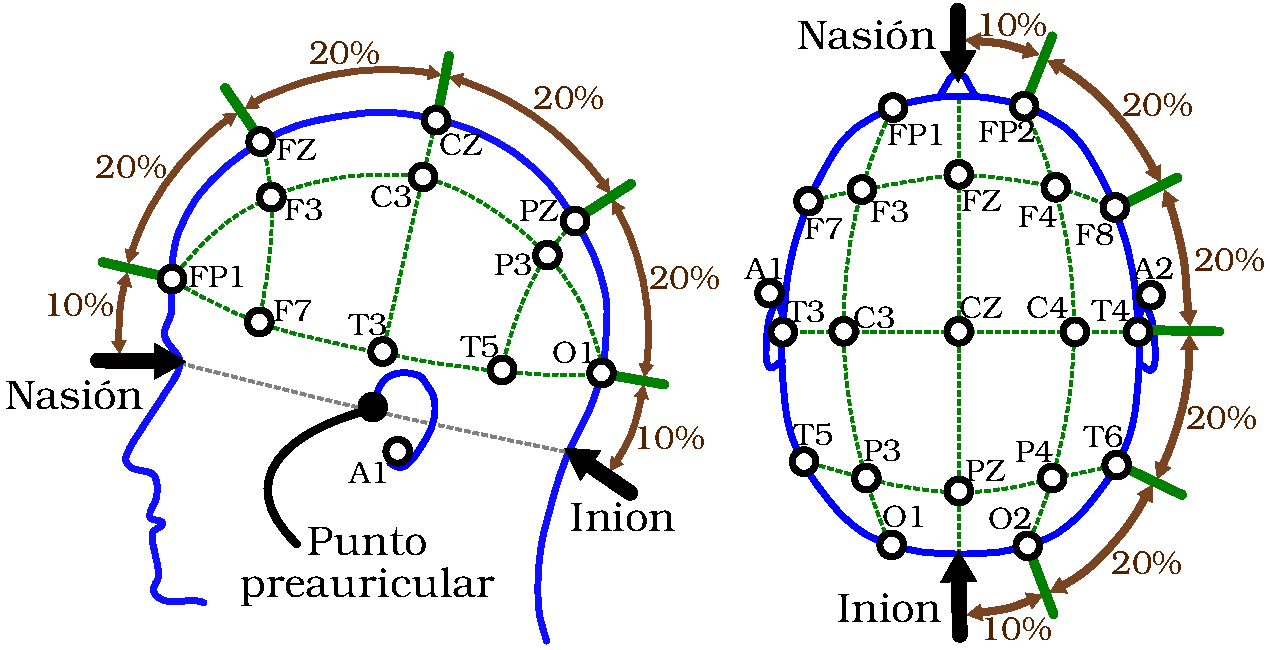
\includegraphics[width=0.9\linewidth]{./img_diagramas/cabeza_hecha.pdf} 
\caption{Colocaci\'on de electrodos seg\'un el sistema 10--20. En el cr\'aneo, el \textbf{inion} es 
una protuberancia craneal, mientras que el \textbf{nasi\'on} es la uni\'on del hueso frontal y los 
huesos nasales; el \textbf{punto preauricular} se ubica arriba del cart\'ilago llamado tragus, que 
protege el canal auditivo \cite{Butkov07}. 
}
\label{img1020}
\end{figure}

Usualmente el EEG muestra una actividad oscilatoria continua y cambiante, cuya 
frecuencia var\'ia entre 0.5 y 100 Hz \cite{Clark98}.
Su composici\'on est\'a fuertemente relacionada con el grado de actividad 
cerebral; por ejemplo, hay diferencias claras durante vigilia y sue\~no.
En general la frecuencia del EEG incrementa cuando hay un altos grados de actividad cerebral, lo 
cual se debe a que las ondas se vuelven m\'as as\'incronas, y entonces la magnitud del  potencial 
integrado de superficie decrece (a pesar de la alta actividad cortical).
Aunque la mayor parte del tiempo el EEG es irregular y no muestra patrones claros, es com\'un que 
muestre ondas cerebrales relativamente organizadas llamadas \textbf{ondas cerebrales} que, 
para su estudio, han sido clasificadas en 
cuatro grandes grupos: alfa, beta, gamma, delta.
Estos grupos son ilustrados en la figura \ref{ritmos}.

\begin{figure}
\centering
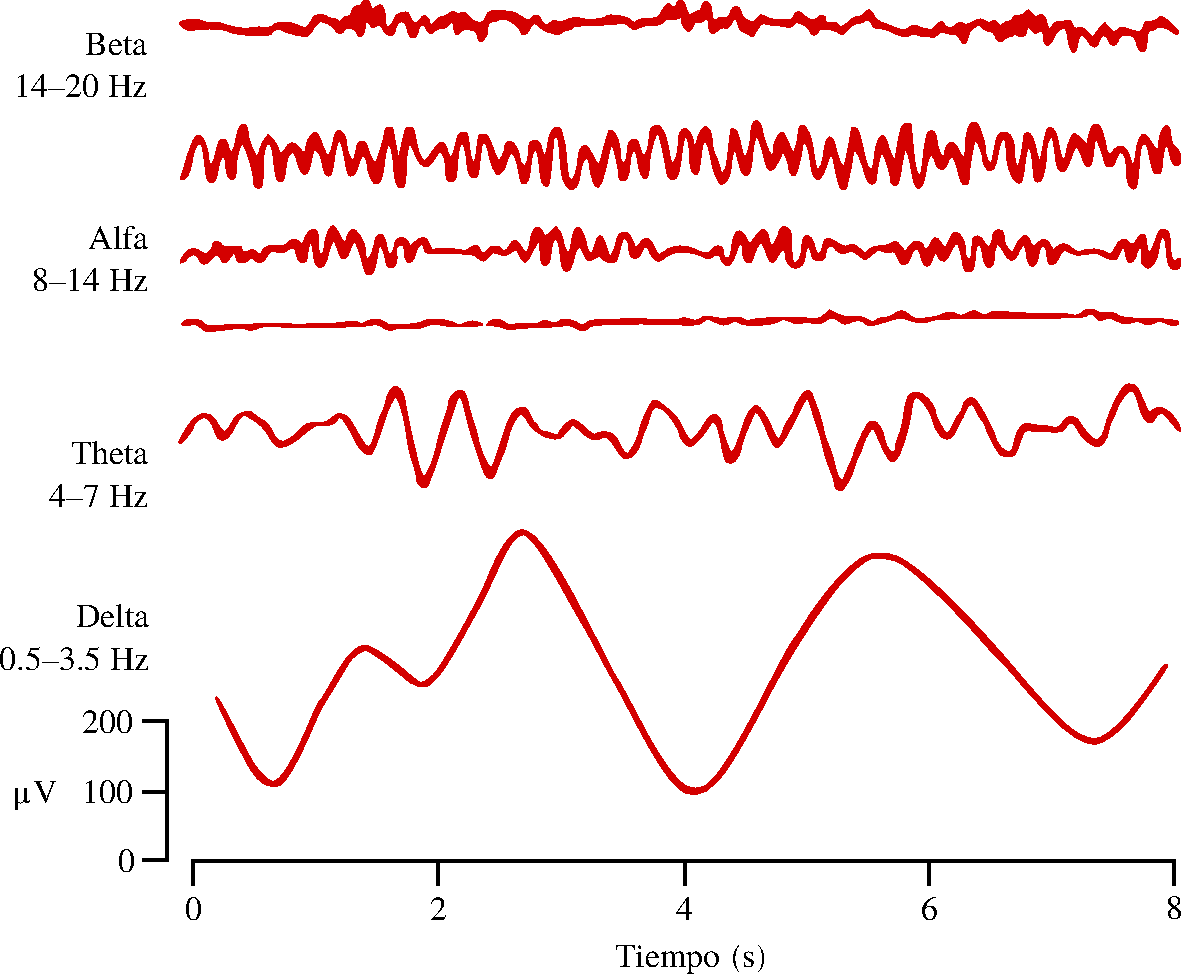
\includegraphics[width=0.55\linewidth]{./img_diagramas/ritmos_hechos.pdf} 
\caption{Ejemplos de ondas cerebrales encontradas en el EEG. Reconstruido de \textit{EEG Signal 
Processing}, por S. Sanei y J. A. Chambers \cite{Sanei07} }
\label{ritmos}
\end{figure}

\begin{description}
\item[Ondas alfa.] Frecuencias entre 8 y 13 Hz. Ocurren en sujetos despiertos en un estado de 
quietud del pensamiento. 
Aparecen m\'as frecuentemente en la regi\'on occipital, pero tambi\'en 
pueden ser registradas en las regiones frontal y parietal. 
%Su voltaje aproximado est\'a entre 20 y 
%200 mV. Cuando el sujeto duerme, las ondas alfa desaparecen completamente. 

\item[Ondas beta.] Frecuencias de 14 a 30 Hz. Normalmente se registran en las regiones parietal y 
frontal. 
%A veces se les divide en dos tipos: beta I y beta II. Las ondas beta I (14--20 Hz) son 
%afectadas por la actividad mental de manera similar a las ondas alfa.
%Las ondas beta II (20--30 Hz), en cambio, aparecen durante una activaci\'on intensa del sistema 
%nervioso central y durante tensi\'on.

\item[Ondas theta.] Frecuencias entre 4 y 7 Hz. Ocurren principalmente en las regiones parietal y 
temporal 
%en ni\~nos, pero pueden aparecer en algunos adultos durante estr\'es emocional, sobre todo 
%durante periodos de decepci\'on y frustraci\'on.

\item[Ondas delta.] Incluye todas las ondas del EEG con frecuencias menores a 3.5 Hz. Ocurren 
generalmente en el sue\~no profundo en infantes, y despu\'es de enfermedades org\'anicas serias del 
cerebro.
\end{description}

Cabe mencionar que el espectro de frecuencias del potencial de campo producido por m\'usculos 
faciales medianamente contra\'idos incluye componentes de frecuencia que bien cuadran en el rango 
usual del EEG (0.5--100 Hz); cuando estas se\~nales 'contaminan' el registro de EEG, son referidas
como \textbf{artefactos}. La variedad de artefactos conocidos es muy basta, al grado de
considerarse a la detecci\'on de \'estos como un paso previo inevitable.

%%%%%%%%%%%%%%%%%%%%%%%%%%%%%%%%%%%%%%%%%%%%%%%%%%%%%%%%%%%%%%%%%%%%%%%%%%%%%%%%%%%%%%%%%%%%%%%%%%%
%%%%%%%%%%%%%%%%%%%%%%%%%%%%%%%%%%%%%%%%%%%%%%%%%%%%%%%%%%%%%%%%%%%%%%%%%%%%%%%%%%%%%%%%%%%%%%%%%%%

\subsection{Sue\~no}

El sueño del ser humano, según criterios polisomnográficos (electroencefalograma, electrooculograma y electromiograma) se divide fundamentalmente en sueño REM (R) (rapid eye movement) y en sueño No REM (NREM)

El sue\~no normal se divide en dos etapas principales: MOR (fase R) y NMOR (fase N), que se 
diferencian por sus rasgos electroencefalogr\'aficos y una serie de caracter\'isticas 
fisiol\'ogicas, y de los cuales obtienen sus nombres.
Cabe mencionar que la nomenclatura acerca de las fases del sue\~no ha sido recientemente modificada 
por la American Association of Sleep Medicine (AASM) en 2007 \cite{AASM07}, de modo que en este 
trabajo se  usar\'an ambas nomenclaturas siempre que sea posible, por fines de compatibilidad.

\begin{description}
\item[Sue\~no] Proceso vital c\'iclico complejo y activo, compuesto por varias fases y que posee 
una estructura interna caracter\'istica, con diversas interrelaciones en los sistemas hormonales y 
nerviosos \cite{FernandezConde07}.
El sue\~no en el ser humano se puede caracterizar por las siguientes 
propiedades\cite{CarrilloMora}:
\begin{enumerate}
\item Disminuci\'on de conciencia y reactividad a est\'imulos externos
\item F\'acilmente reversible (lo cual lo diferencia de otros estados 
patol\'ogicos como el estupor y el coma)
\item Inmovilidad y relajaci\'on muscular
\item Periodicidad t\'ipica circadiana (diaria)
\item Los individuos adquieren una postura estereotipada
\item La privaci\'on induce alteraciones conductuales y 
fisiol\'ogicas, adem\'as de que genera una 'deuda' acumulativa
\end{enumerate}
\end{description}

Durante el sue\~no MOR (fase R), ocurre que las ondas lentas y amplitud alta son reemplazadas por 
ondas r\'apidas de bajo voltaje, irregulares, y que recuerdan la actividad en el EEG durante el 
estado de alerta.
La presencia de estos patrones irregulares no interrumpen el sue\~no, sino que incrementan el 
umbral para los est\'imulos externos; este comportamiento es referido como 'sue\~no parad\'ojico'.
Durante esta etapa de sue\~no, el sujeto exhibe movimientos oculares r\'apidos (MOR), raz\'on por 
la cual recibe su nombre caracter\'istico.
Durante el sue\~no MOR se producen la mayor\'ia de las enso\~naciones (referidos coloquialmente 
como sue\~nos), y la mayor\'ia de los pacientes que despiertan durante esta fase suelen recordar 
v\'ividamente el contenido de sus enso\~naciones \cite{Chokroverty09}.
F\'isicamente el tono de todos los m\'usculos disminuye (con excepci\'on de los m\'usculos 
respiratorios y los esf\'interes vesical y anal), as\'i mismo la frecuencia cardiaca y respiratoria 
se vuelve irregular.

El sue\~no fuera de la etapa MOR es referido como no-MOR (NMOR, fase N), y es dividido en etapas 
seg\'un la 'profundidad' del sue\~no, entendida en t\'erminos de la actividad cerebral registrada.
En el sue\~no profundo se observan ondas delta muy irregulares, y junto con ellas ocurren trenes 
cortos de ondas, parecidas a las alfa, y que son referidas como \textit{husos de sue\~no}. 
El ritmo alfa y los husos de sue\~no est\'an sincronizados en el sue\~no y la somnolencia, en 
contraste con la actividad irregular, desincronizada y de bajo voltaje registrada en estado de 
alerta.
A grosso modo, la clasificaci\'on de etapas del sue\~no seg\'un la AASM se basa en las siguientes
caracter\'isticas \cite{Hori01}:

\begin{description}
\item[Vigilia (W)] Presencia de ritmo alfa contin\'uo con m\'axima amplitud sobre regiones de la 
corteza parieto-occipital. Tono muscular relativamente alto y ausencia de movimientos oculares.

\item[Fase 1 (N1)] Corresponde con la somnolencia o el inicio del sue\~no ligero, en ella es muy 
f\'acil despertarse. 
Presencia intermitente de ondas alfa en menos del 50\% de la \'epoca, actividad de frecuencias 
mezcladas y bajo voltaje, adem\'as de movimientos oculares lentos y algunas ondas agudas. 
La actividad muscular disminuye paulatinamente, pueden observarse sacudidas musculares s\'ubitas 
que a veces coinciden con una sensaci\'on de ca\'ida. 

\item[Fase 2 (N2)] Se caracteriza por patrones espec\'ificos de actividad cerebral conocidos como 
husos de sue\~no y complejos K. 
Puede aparecer hasta un 20\% de ondas lentas (ritmo delta). Ausencia de actividad ocular y tono 
muscular bajo.
La temperatura, la frecuencia card\'iaca y respiratoria disminuyen paulatinamente. 

\item[Fases 3 (N3)] Predominan ondas de frecuencias muy bajas ($<2$ Hz) con amplitudes superiores a 
75 $\mu$V en m\'as del 20\% y menos del 50\% de la \'epoca. Pueden tambi\'en aparecer complejos K y 
husos de sue\~no de forma espor\'adica. Ausencia de actividad ocular y tono muscular bajo.

\item[Fase 4 (N4)] La fase m\'as profunda del sue\~no NMOR y referido como 'sue\~no de ondas 
lentas', pues hay presencia de \'estas ondas en m\'as del 50\% de la \'epoca. Las dem\'as 
caracter\'isticas son similares a las de la fase 3.

\item[Fase MOR (R)] Presencia de actividad EEG de baja amplitud y frecuencias entremezcladas 
(theta-alfa-beta) similar a la observada en el estado de vigilia activa con ojos abiertos.
\end{description}

Un adulto joven pasa aproximadamente entre 70--100 minutos en el sue\~no NMOR para despu\'es entrar 
al sue\~no MOR, el cual puede durar entre 5--30 min; este ciclo se repite cada hora y media.
En los ancianos se va fragmentando el sue\~no nocturno con frecuentes episodios de despertar, se 
reduce mucho el porcentaje de sue\~no en fase 4, pero se mantiene constante el porcentaje de 
sue\~no MOR. Adicionalmente, muchos adultos mayores dormitan durante el d\'ia varias siestas cortas 
\cite{CarrilloMora}.

La edad es un factor decisivo para la cantidad de horas de sueño. El recién nacido duerme entre 14 y 18 horas, el lactante entre 12 y 14 horas, el niño en etapa escolar entre 11 y 12 horas y en la edad adulta, la mayoría duerme entre 7 y 8 horas por noche. En otras palabras, es fisiológico que el número de horas dormidas vaya disminuyendo progresivamente a lo largo de la vida, pudiendo existir una diferencia de hasta 16 horas como promedio entre la niñez y la edad adulta. En los ancianos, el número de horas de diferencia entre las horas de sueño propias v/s las horas de sueño de la niñez, es aún mayor

\cite{Contreras13}

%%%%%%%%%%%%%%%%%%%%%%%%%%%%%%%%%%%%%%%%%%%%%%%%%%%%%%%%%%%%%%%%%%%%%%%%%%%%%%%%%%%%%%%%%%%%%%%%%%%
%%%%%%%%%%%%%%%%%%%%%%%%%%%%%%%%%%%%%%%%%%%%%%%%%%%%%%%%%%%%%%%%%%%%%%%%%%%%%%%%%%%%%%%%%%%%%%%%%%%
%%%%%%%%%%%%%%%%%%%%%%%%%%%%%%%%%%%%%%%%%%%%%%%%%%%%%%%%%%%%%%%%%%%%%%%%%%%%%%%%%%%%%%%%%%%%%%%%%%%
%%%%%%%%%%%%%%%%%%%%%%%%%%%%%%%%%%%%%%%%%%%%%%%%%%%%%%%%%%%%%%%%%%%%%%%%%%%%%%%%%%%%%%%%%%%%%%%%%%%
